\documentclass[a4paper,11pt]{article}
%\usepackage[T1]{fontenc}

%\setlength{\textwidth}{20cm}
%\setlength{\marginparwidth}{0cm}
%\setlength{\voffset}{0cm}
\usepackage[utf8]{inputenc}
\usepackage[francais]{babel}
\usepackage{amsmath}
\usepackage{graphicx}

%\special{papersize=210mm,297mm}

\title{{\Huge Electronique numérique}\\Chemins de données ou {\it datapath}}
\date{}

\begin{document}
\maketitle
{\it Tous les exercices ne seront pas forcément résolus en TE.}

\section{Notion de chemin de données ou {\it datapath}}

Nous avons déjà abordé le notion de "chemins de données"  dans le "jeu des cambrioleurs" : il s'agissait
uniquement d'acheminer, en combinatoire, une donnée d'une entrée vers une sortie, sans traitement spécifique. En général, les "datapath" sont plus complexes
et associent à la fois logique séquentielle et logique combinatoire. Les datapaths permettent d'effectuer des calculs rapides. L'essentiel de leur puissance
de calcul provient de deux notions fondamentales :
\begin{itemize}
  \item Le \textbf{parallélisme} : il s'agit d'effectuer plusieurs opérations durant 1 seul cycle d'horloge, grâce à l'utilisation de plusieurs opérateurs matériels.
  Pour rappel, dans un processeur classique (et comme dans les langages dits "séquentiels"), les opérations se font en séquence, les unes à la suite des autres. Ici, à l'inverse,
  nous sommes en mesure de construire des calculateurs qui effectuent plusieurs opérations simultanément.
  \item Le \textbf{pipeline} : il s'agit d'effectuer des opérations "à la chaîne", sur des données, chaque {\it étage} du pipeline ayant une action spécifique sur ces données.
  Nous allons d'abord chercher à illustrer le rôle de la bascule D dans la structure d'un pipeline élémentaire : le registre à décalage.
\end{itemize}


\section{Pipeline, Registres à décalage et Applications}
Le registre à décalage le plus simple consiste à relier la sortie d'une première bascule D à l'entrée d'une seconde bascule D.
Ceci se généralise à un nombre $L$ de bascules ainsi enchaînées les unes aux autres (sans rebouclage).
Une donnée $e$ qui se présente au cycle $n$ mettra $L$ cycles (ou "coups d'horloge") à parvenir à la sortie $s$.
Sa fonction est double :
\begin{enumerate}
  \item Retarder  la donnée $a_0$ d'un temps discret $L$ : elle se présente sur l'entrée $e$ au temps $t$ et ressort sur la sortie $s$ du dispostif au temps $t+L$.
  \item Autoriser une donnée $a_1$ à se présenter sur l'entrée $e$ au temps $t+1$, en même temps que $a_0$ est échantillonnée par la seconde bascule, etc.
\end{enumerate}

\paragraph{Exercice 1 : registre à décalage simple} Dessiner un registre à décalage de taille 4. Nommer correctement ses signaux et écrire l'équation de la sortie $s(t)$.\\
\paragraph{Exercice 2 : registre à décalage commandé} Modifier le registre à décalage précédent de manière à le commander par un signal 'push', qui autorise les données à s'acheminer progressivement vers la sortie lorsque ce signal
vaut '1'.\\

% \paragraph{Exercice 2 : FIFO} Une FIFO ({\it first-in, first-out}) est une structure de données (matérielle ou logicielle), qui permet de stocker des données dans l'attente d'un traitement par
% un processus (ici un circuit). L'ordre d'arrivée des données est préservé. La FIFO possède également un signal booléen {\it push} qui donne d'ordre à la FIFO s'accepter une nouvelle entrée, et qui
% contrôle globalement le pipeline.

\paragraph{Exercice 3 : moyenne mobile} Soit un flux séquentiel de données (boursier, médical, etc), dont les données successives arrivent au rythme de 100 Mhz.
La moyenne mobile (ou moyenne glissante, ou {\it sliding average} en anglais) d'un tel flux continu permet de lisser une moyenne au cours du temps.
\begin{enumerate}
  \item Calculer rapidement la moyenne mobile, sur 4 échantillons, du flux suivant : $$...,0,0,0,0,8,9,13,4,3,2,1,0,0,0,....$$
  \item Concevoir un circuit numérique qui réalise le calcul d'une moyenne mobile sur 4 échantillons de nombres entiers, supposés non signés. Proposer une seconde solution. Laquelle est meilleure ?
  On s'autorise à utiliser la notion d'additionneur, mais pas de diviseur.
  \item Combien de bits sont nécessaires pour calculer la somme de $4$ données codées sur $8$ bits ?  Combien pour la moyenne mobile ?
  \item Combien de bits sont nécessaires pour calculer la somme de $n$ données codées sur $m$ bits ?
  \item Sachant que le temps de traversée de l'additionneur est 4 ns, quelle est la fréquence atteignable du circuit ? Est-ce compatible avec la fréquence d'arrivée des données ?
\end{enumerate}

% \begin{figure}[!h]
%   \centering
%   \fbox{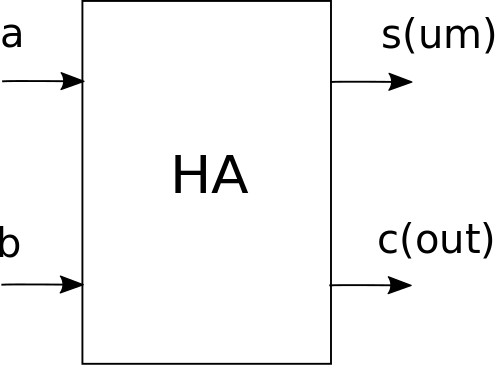
\includegraphics[scale=0.4]{ha.png}}
%   \caption{Circuit ('netlist') du demi-additionneur 1 bit}
%   \label{ha}
% \end{figure}

\paragraph{Exercice 4 : look-up table de FPGA} Les FPGA sont des circuits réguliers qui ont l'étonnante propriété d'être
reprogrammables à volonté. On parle de "circuits reconfigurables".
Les FPGA sont constitués d'un assemblage de briques élémentaires appelées BLE (Basic Logic Element), interconnectées en réseau.
Leur topologie détaillée est présentée dans le polycopié du cours. Un BLE se compose notamment d'une
LUT (look-up table) à $n$ entrées : c'est une mémoire qui permet d'enregistrer
les valeurs attendues de n'{\it importe quelle fonction booléenne à n entrées}.
C'est l'équivalent matériel d'une petite table de vérité, qui se présente sous la forme d'un registre à décalage {\it avec 'enable'} (voir exercice précédent où on a appelé ce signal 'push')
\footnote{...pour les besoins de
notre exercice. Les LUTs des FPGAs sont réalisées au niveau transistors.}
à $2^n$ bascules : le flux qui entre dans ce registre à décalage s'appelle un {\it bitstream}.
Il agit comme une programmation  ou {\it configuration} de la LUT.
Chaque sortie $Q_i$ des bascules de la LUT est connectée à une des $2^n$ entrées d'un multiplexeur.
Les signaux de contrôle du multiplexeur sont les $n$ entrées, notées ici $\{a,b,c,\dots,\alpha_{n-1}\}$.

\begin{enumerate}
  \item Dessiner une LUT 2.
  \item On suppose que le bitstream est entré à l'aide d'un signal de contrôle auxiliaire 'push' (cf exercice 2) de la manière suivante : $1000$, où le bit le plus à droite représente la première
  donnée. Calculer la sortie du multiplexeur pour les combinaisons des entrées $a,b$.
  \item Quelle est la fonction réalisée par le dispositif ?
  \item Conclure en proposant un bitstream pour la fonction $xor(a,b)$.
\end{enumerate}

\section{Exo 5 : Pipeline et datapath}

On cherche à concevoir un calculateur qui réalise l'opération arithmétique complexe $y=a*b*c*d$ en un seul cycle d'une horloge à 100 Mhz. Les données $a,b,c,d$ sont codées sur 8 bits et stockées
au préalable dans des bascules D (appelées registres). Le résultat $y$ est également stocké dans un registre.

\begin{enumerate}
  \item Sur combien de bits est-il nécessaire de stocker $y$ ?
  \item Dessiner une première architecture, purement combinatoire.
  \item Sachant que le temps de traversée d'un multiplieur est de 4 ns, quelle est la fréquence maximum de fonctionnement du calculateur ? Respectez vous le cahier des charges ?
  \item Catastophe ! Le temps de traversée du multiplieur est finalement revu à la hausse : 6 ns. Pouvez-vous corriger le circuit ? Respectez vous encore le cahier des charges ?
\end{enumerate}


\end{document}
